%!TEX root = project.tex

\chapter{Technology Review}
About seven to ten pages.
\begin{itemize}
    \item Describe each of the technologies you used at a conceptual level. Standards, Database Model (e.g. MongoDB, CouchDB), XMl, WSDL, JSON, JAXP.
    \item Use references (IEEE format, e.g. [1]), Books, Papers, URLs (timestamp) – sources should be authoritative.
\end{itemize}

\begin{figure}[H]
    \centering
    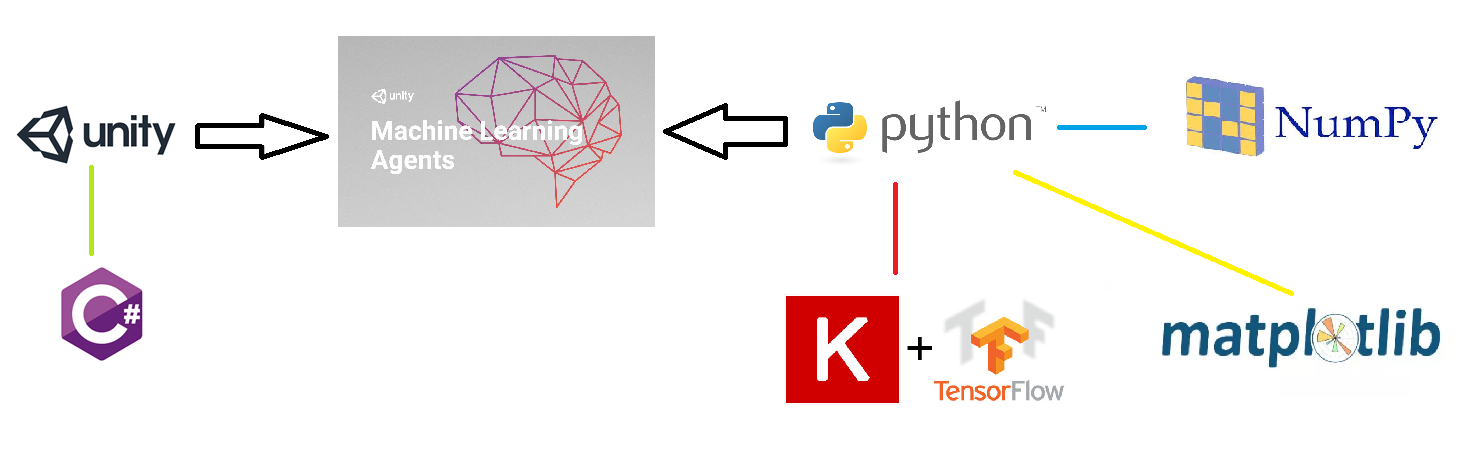
\includegraphics[width=130mm, height=35mm]{img/TechUsed.png}
    \caption{Technologies used}
    \label{fig:sd4}
\end{figure}

\section{Machine Learning}
Machine learning (ML) is an application of artificial intelligence (AI) that provides systems the ability to automatically learn and improve from experience without being explicitly programmed. Machine learning focuses on the development of computer programs that can access data and use it learn for themselves.

One of the current trends in modern day software development is the exploration into the world of Artificial intelligence.
With the recent boom of Artificial Intelligence and Machine learning, we thought it would be a good idea to jump onto the bandwagon and see what it was all about.
In this paper we will describe in detail our process of creating an unity environment with the goal of teaching an agent how to play soccer, the challenges encountered throughout and the research done into the areas of Machine Learning and the Unity environment.  We will then discuss how we implemented this idea with ideas acquired from our research. We will then discuss our results, what we learned and how we could possible improve on in the future with further research.

\section{Neural Networks}
Neural network, a computer program that operates in a manner inspired by the natural neural network in the brain. The objective of such artificial neural networks is to perform such cognitive functions as problem solving and machine learning.
\section{Unity}
Unity is a cross-platform real-time engine developed by Unity Technologies. The engine can be used to create both three-dimensional and two-dimensional games as well as simulations for its many platforms.
\section{Python}
Python is an interpreted, object-oriented, high-level programming language with dynamic semantics. Its high-level built in data structures, combined with dynamic typing and dynamic binding, make it very attractive for Rapid Application Development, as well as for use as a scripting or glue language to connect existing components together. Python's simple, easy to learn syntax emphasizes readability and therefore reduces the cost of program maintenance. 

\section{Jupyter Notebook}
Notebooks
Through the use of the Jupyter notebook, we could develop our AI through python while also documenting it in a nice style with the use of the Markdown option. This provided a clear user-friendly experience when running the python code through the notebook with in depth explanations of what our code does. The Jupyter notebook app is a server to client application that allows users to create notebook documents and run then via the web browser. This app can be run on a local desktop without the requirement of internet access through the command line. There is also a similar version of this web app called Jupyter Lab. This version of the web app grants the user a more IDE-like experience, allowing the user to have many tabs in the same window. With our development we went with using the Jupyter Lab version over the Jupyter Notebook version as we found it more useful due to the number of notebooks we would be developing and the GUI similar to an IDE made it more comfortable to work in. 

To open the Jupyter notebook version of the web application, enter the following into the command line
\begin{minted}{console}	
	Jupyter notebook 
\end{minted}
To open the Jupyter lab version of the web application, enter the following into the command line
\begin{minted}{console}
	Jupyter lab 
\end{minted}

%Look at this again - Ryan
\subsection{How it works}
The notebooks are broken up into individual cells. Each individual cell can be specified into three different types of syntax: Markdown, Python and Raw text. Below is an example of both a Markdown and a python cell taken from our project before they are executed.

\begin{figure}[H]
    \centering
    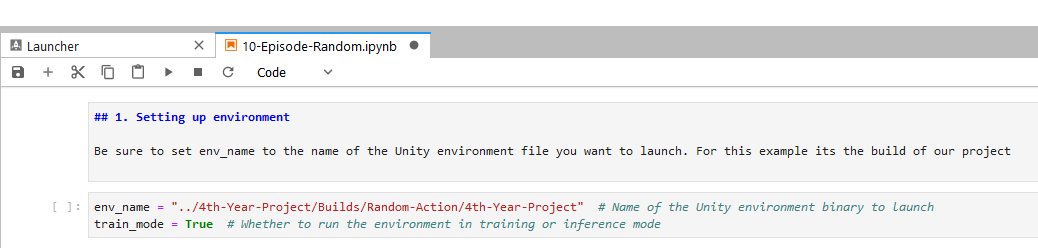
\includegraphics[width=115mm, height=30mm]{img/Notebook1.PNG}
    \caption{Notebook cells before execution}
    \label{fig:sd4}
\end{figure}

\begin{flushleft}
As you can see the first cell block contains the markdown syntax and the second cell containing python syntax before they have been executed.
\end{flushleft}

\begin{figure}[H]
    \centering
    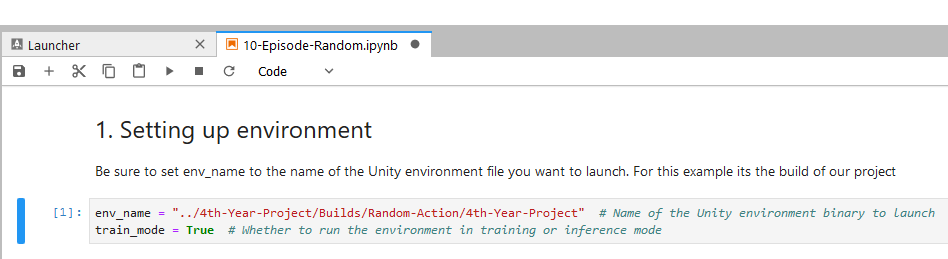
\includegraphics[width=115mm, height=30mm]{img/Notebook2.PNG}
    \caption{Notebook cells after execution}
    \label{fig:sd4}
\end{figure}

\begin{flushleft}
In this image we see both cells after being executed. The number "1" to the left of the cell indicates that this has finished running and its the first python cell that has been executed in the notebook. 
\end{flushleft}

%end

Technologies Review:
This chapter will discuss in detail the technologies that we utilised in the project. It will also provide examples of the research we did into the different types of possible technologies. It will also highlight the rationale behind the decisions we made to use certain technologies over others.

Game Engines:
In this section, we will discuss the possible game engines we can use to run our environment in. We don't want to try use actual hardware and would prefer to run our environment in a game engine.

Unity

Unity is a real-time game engine developed by Unity Technologies and released back in June of 2005. Originally designed as an OSX-excluseive game engine, the software has been developed upon and extended to support a host of other platforms also. Unity has made a name for itself, making game development accessible to everyone, as shown by the sheer amount of indie game developers using Unity as there main game engine tool.

Why use Unity
The main pull Unity has over other game engines is it's ease of use, the software has been designed to make it easy to design games from the ground up, with easy to understand UI and an overall aim to create functional, smart, and sometimes simple games, rather than complex games with high quality graphics. Also the fact that the software is free to download and use is a big plus.

Unreal Engine
Unreal Engine was developed alongside it's debut title "Unreal" in 1998 by Epic Games. The game engine has kept a reputation of it being a high end piece of software, both due to it's price plans, and it's ability to generate incredible graphics.

Why use Unreal
The software has had some problems in the past with it's steep learning curve. Certainly not a beginners piece of software, however if someone who has had previous experience with coding and other 3d programs is looking to create a highly detailed expansive game, they need look no further than Unreal Engine.

Our decision
We decided to use Unity over Unreal Engine, firstly because of the learning curve. We had the opportunity to use Unity previously in a module, so we all had a slight bit of experience. Also the fact Unity is completly free, whereas Unreal Engine requires a payment plan to be set up, was what finally sold us on using Unity.


Neural Network Languages:
In this section we will discuss the different languages we reviewed to write our neural network in. The following programming languages have all been noted as strong languages for neural network design.

Python
Created by Guido van Rossum, Python is a high level, general purpose programming language first released in 1991. Pythons design philosophy emphasizes code readability, meaning the language utilises a significant amount of white space. The language supports multiple programming paradigms, so programs written procedurally will work just as well as an object oriented program design.

Why Python 
Simplicity is a major factor when talking about neural network design, so having a language that's easy to understand, aswell as the fact that python has an extreamly large library of useful framworks to utilise makes it a very strong choice.

R
R is a programming language and software environment used for statistical computing, and is great for producing informative graphics and data mining. Origionally introduced back in 1993, the language has stuck around due to it's presence as a truely general purpose programming language.

Why R
Although R doesn't originally apear to be a language that would suit neural network design, the sheer amount of libraries that R boasts, including RODBC, Gmodels, and Tm, which are all used in the field of machine learning, means the language actually has a strong case for being the correct one to use.

Lisp
Lisp is a family of programming languages, originally specified way back in 1958. It is the second oldest high level programming language that is still in widespread use today. John McCarthy, the inventor of the language, is actually known as the father of Artificial Intelligence, and many of the languages features have been inplimented and migrated over into more modern programming languages.

Why Lisp
Apart from it's inventor harolding the title of the father of AI, Lisp actually became the favoured language for AI development and research shortly after it's introduction.

Our decision
We decided to use Python as our language to build the neural network in due to the fact that the language is currently considered to be on top when it comes to AI development. Even though R and Lisp both were strong candidates for what language to use, the fact that Python is designed to be so simplistic and easy to understand made it the best choice for us, as we would need to be able to get our heads around the inner workings of neural networks quickly.

Connector Software:
In this section we will discuss the possible ways to connect the neural network code to the game engine environment.

Jupyter Notebooks
The Jupyter Notebook App is a server-client application that allows the editing and running of notebook documents via a web browser. Notebook documents are produced by the App and can contain both computer code aswell as rich text elements. These documents acts as executables which can run whatever code they consist of.

Why Jupyter Notebooks
We have had previous experience with notebooks, using them in a previous module, so we already have an understanding of their inner workings. We also found plenty of examples of other people connecting game engine environments to  external code. Having a previous understanding of the ins and outs of these notebook documents will be a great advantage to using notebooks as a connector between the environment and external code.


Transmission Control Protocol connection
TCP is one of the main protocols of the Internet protocol suite. TCP provides a reliable, ordered, and error-checked delivery of a stream of bytes between applications communicating via an IP network. 

Why Transmission Control Protocol
A TCP connection has been attempted to connect a game engine environment to external neural network code by others. We found some examples of other attempts, with some positive results. The bonus to using a TCP connection would be the fact that literally anything could be passed between the environment and the external code. Json objects could be passed back and forth meaning any input needed for the neural network, and subsequent output, could all be passed back and forth with ease, once a connection between the two had been established.

\section{XML}
Here's some nicely formatted XML:
\begin{minted}{xml}
<this>
  <looks lookswhat="good">
    Good
  </looks>
</this>
\end{minted}